\section{Rappresentazione della Conoscenza}
Generalmente la conoscenza musicale di ogni musicista, cantante,
compositore o direttore d'orchestra è formata da tre 
componenti fondamentali:
\begin{enumerate}
\item esecuzioni passate dell'artista stesso
\item esecuzioni altrui ascoltate precedentemente
\item regole provenienti dalla teoria musicale
\end{enumerate}

In IMprovEEsation queste informazioni sono alla base del modello della
conoscenza degli agenti del sistema. Le componenti 1 e 2 costituiscono i
pattern musicali e le relative note associate ad essi. Inoltre nella memoria
degli agenti sono presenti informazioni aggiuntive, come ad esempio
scale, modo degli accordi, etc. Queste ultime vengono messe in relazione
con i pattern e le note formando così la terza componente, ovvero l'insieme 
di regole teoriche possedute dall'agente.\\ 
Inoltre la conoscenza degli agenti viene rappresentata come se fosse 
immagazzinata in un unica memoria collettiva, che viene acceduta però in
regioni diverse in base al ruolo dell'agente. Ad esempio il direttore ha
accesso alla regione della memoria dove sono salvate le informazioni
riguardo all'andamento complessivo di un improvvisazione che comunicherà
durante quest'ultima ai musicisti. Un agente musicista ha accesso alla
regione di memoria dove salvate le informazioni necessarie per comporre
in tempo reale delle note che siano coerenti in qualche modo con le
informazioni fornite dal direttore.
\subsection{Pattern e Regole}
\label{patterneregole}
% XXX MATTE XXX %
Definiamo i pattern come sequenze di misure di accordi. 
Il direttore ha la conoscenza di una collezione di diversi pattern che
a loro volta possono ammettere delle varianti di dinamica e stile.
%TODO: spiegare meglio la struttura del pattern %
Il musicista, nella memoria complessiva, ha accesso alle collezioni di
informazioni riguardo note singole. 
Si è scelto di rappresentare una singola nota come una semicroma essendo 
1/16 la suddivisione temporale più piccola che prendiamo in considerazione.
Inoltre ad ogni semicroma non è associato un solo valore tonale, ma un
vettore di probabilità ($pnotes$) di dimensione $n$ pari a 13. L'indice i-esimo
di ogni elemento corrisponde alla distanza tonale dalla tonalità, 
Key Signature $KS$, decisa dal direttore, oppure una pausa (indice 0). 
Ogni elemento i-esimo del vettore 
corrisponde al valore di probabilità $p_i$ che la nota $nt_i$ di distanza 
$i$ dalla $KS$, venga selezionata rispetto alle altre.
\[nt_i = i + KS \]
\[p_i = \text{probability to choose  } nt_i \]
\begin{equation}
\label{eq-pnotes}
pnotes = (p_0, p_1,  \ldots , p_i, \ldots, p_n)
\end{equation}
Inoltre i valori $p_i$ contenuti nel vettore $pnote$ formano una distribuzione 
(arbitraria) di probabilità in quanto vale:
\begin{equation}
\sum_{i=0}^{n} p_i = 1 \;\;\;\; p_i \in [0, 1]
\end{equation}

Per ogni semicroma è associato anche un valore di probabilità $p_c$
utilizzato per decidere se quella semicroma e il suo vettore di
probabilità debba essere considerato ad un certo istante di tempo $t$.
Nella memoria del musicista sono presenti anche i quarti che raggrupprano 
fino a 4 semicrome ognuno. Ai quarti sono correlate ulteriori informazioni, utili
a comprendere il contesto di appartenenza di un certo quarto, come:
\begin{itemize}
\item posizione del quarto in una misura
\item l'accordo associato
\item il modo dell'accordo 
\item strumento associato
\item dinamica del quarto
\item mood (stile) del quarto
\item se lo strumento associato è solista o meno
\end{itemize}
Mettendo in relazione queste informazioni con quelle fornite dal
direttore durante un improvvisazione, un musicista cerca di 
scegliere delle note che siano il più possibile inerenti al contesto.
Come ciò viene fatto verrà spiegato nella sezione \ref{thinking}.
\subsection{Database Relazionale}
\label{database}
% XXX MATTE XXX %
\begin{figure}[H]
\centering
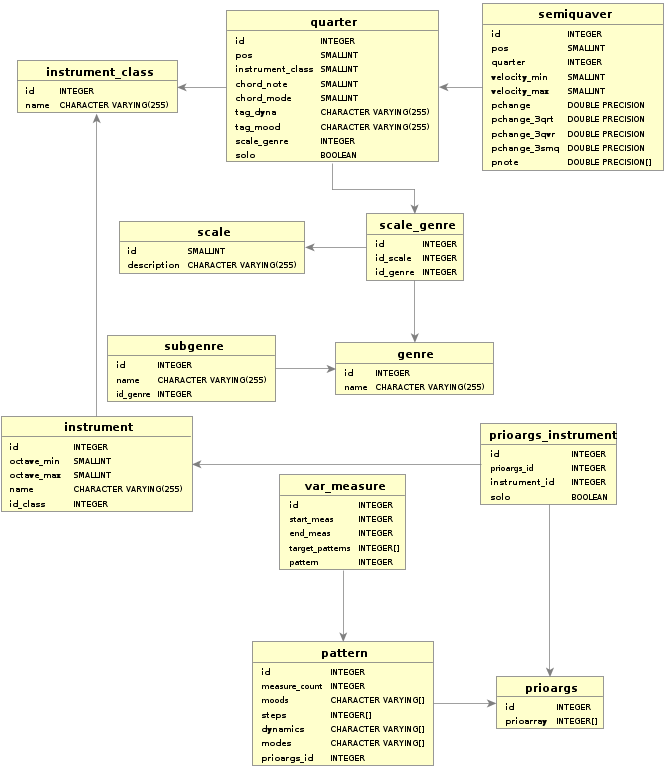
\includegraphics[scale=0.7]{img/db.png}
\caption{Schema E-R del DataBase}
\label{figure-db}
\end{figure}
La struttura di conoscenza spiegata nel paragrafo precedente è stata implementata
tramite un DataBase relazionale il cui schema Entitià Relazione è mostrato nella figura
\ref{figure-db}.\\
La struttura si può pensare come divisa essenzialmente in due parti principali.\\ 
La prima si concentra intorno alla tabella $quarter$, attraverso la quale il musicista
riesce a capire quali $semiquaver$ considerare in base ad un certo contesto definito
dal direttore come già spiegato nella sezione precedente. È importante notare che 
nonostante la memoria sia collettiva a tutti gli agenti, tramite le informazioni 
legate ai quarti un musicista è in grado di filtrare le informazioni che meglio si
adattano a se stesso. Oltre al contesto definito dal direttore infatti, il musicista
può anche filtrare le informazioni che riguardano la sua natura, come ad esempio 
il tipo di strumento da lui suonato o se si sta comportando o meno da solista.\\
La seconda parte fondamentale del DataBase è concentrata intorno alla tabella $pattern$.
Dalla figura \ref{figure-db} potrebbe sembrare che l'entità $pattern$ non abbia poi 
così tante relazioni come l'entità $quarter$ per considerare quest'utlima un parte
fondamentale del DB. Questo deriva dal fatto che si è deciso di semplificare un po'
il modello E-R per l'entità $pattern$ utilizzando dei vettori per ogni record di 
quest'ultima anzichè creare delle nuove entità-relazioni. Questa scelta è giustificata
dal fatto che viene inizialmente considerato un numero relativamente basso di pattern
e che il modello è facilemente estendibile in quanto le due parti fondamentali del 
DataBase hanno due schemi abbastanza indipendenti tra loro.\\
Nello specifico la tabella $pattern$ è caratterizzata fondamentalmente dai 
seguenti campi vettoriali
\begin{itemize}
\item steps 
\item modes 
\item dynamics
\item moodes
\end{itemize}
tramite i quali un direttore riesce a scandire l'andamento dell'improvvisazione 
misura per misura, definendo a quali accordi riferirsi e suggerendo ai musicisti 
con quale dinamica e "sentimento" eseguire le loro perfomance. Queste direttive
possono venire suggerite ai musicisti in modo stretto o lato.\\
A tal proposito ad ogni pattern viene associato un vettore di priorità dalla tabella 
prioargs che definisce con quale priorità le direttive del direttore riguardanti quel 
pattern debbano essere considerate dai musicisti, anche rispetto alle altre 
informazioni sulla loro stessa natura. È anche possibile che un musicista non consideri
affatto le priorità legate al pattern ma utilizzi delle priorità ad-hoc, definite 
rispetto ad altri parametri.\\
Ad esempio un musicista solista potrebbe considerare un vetttore di priorità 
ad-hoc che non sia legato a nessun pattern in quanto 
potrebbe non essere interessato alla successione di accordi tra le misure, 
informazione molto forte per i pattern, ma solamente alla tonalità corrente, 
alle dinamiche e ai mood delle misure.\\
C'è poi il caso particolare del batterista
che non ha alcun interesse riguardo le informazioni inerenti alla linea melodica 
e aromica di un improvvisazione, ma è interessato solo alla linea ritmica. Inoltre
per il batterista viene utilizzato un modello diverso di vettore di probabilità 
di ogni semiquaver, quindi è fondamentale che la sua priorità più alta sia il tipo 
di strumento, altrimenti, incorrenendo in vettori di priorità associati a quarti di
altri strumenti, potrebbe interpretare in maniera completamente errata tali informazioni.\\\\
Dal lato applicazione le informazioni residenti nel DB vengono recuperate tramite
una libreria dinamica dedicata. Quest'ultima si occupa di effettuare le apposite
query per recuperare le informazioni, con i dovuti vincoli, necessarie ai processi 
musicisti e direttori per improvvisare.
